
\begin{figure}[H]
\centering
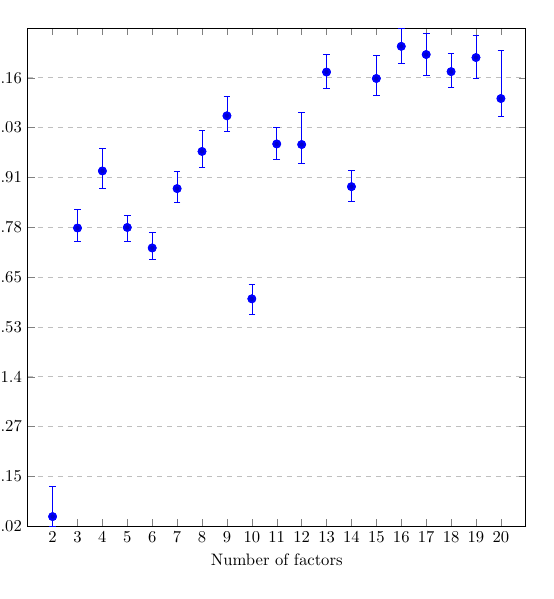
\begin{tikzpicture}[scale=0.6, trim axis left, trim axis right]
\begin{axis}[
    width=1\textwidth,
    height=1\textwidth,
    xlabel={Number of factors},
    ylabel={Time taken (s)},
    xmin=1.0, xmax=21.0,
    ymin=1.01826, ymax=2.287249,
    xticklabels={2, 3, 4, 5, 6, 7, 8, 9, 10, 11, 12, 13, 14, 15, 16, 17, 18, 19, 20},
    xtick={2, 3, 4, 5, 6, 7, 8, 9, 10, 11, 12, 13, 14, 15, 16, 17, 18, 19, 20},
    ytick={1.01826, 1.1451589, 1.2720578, 1.3989567, 1.5258556, 1.6527545, 1.7796534, 1.9065523, 2.0334512, 2.1603501},
    ymajorgrids=true,
    grid style=dashed,
]

\addplot+[
    blue,
    very thick,
    forget plot,
    only marks
    ]
    plot[
    very thick,
    error bars/.cd,
    y dir=plus,
    y explicit
    ]
    table[x=x,y=y,y error expr=\thisrow{y-max}] {
    x    y    y-max
    11	1.9919114	0.0415456
10	1.59734733333	0.0360946666667
13	2.17506696667	0.0449480333333
12	1.9904225	0.0819875
15	2.1586458	0.0591132
14	1.8831095	0.0412595
17	2.2197465	0.0536575
16	2.24052783333	0.0467211666667
19	2.21200643333	0.0571895666667
18	2.1760707	0.0471053
20	2.10760823333	0.123275766667
3	1.77776056667	0.0463764333333
2	1.04261126667	0.0767157333333
5	1.7791179	0.0317951
4	1.92306296667	0.0577200333333
7	1.87813433333	0.0443016666667
6	1.726933	0.040735
9	2.06360606667	0.0484439333333
8	1.9727841	0.0537149

    };

\addplot+[
    blue,
    very thick,
    forget plot,
    only marks
    ]
    plot[
    very thick,
    error bars/.cd,
    y dir=plus,
    y explicit
    ]
    table[x=x,y=y,y error expr=\thisrow{y-min}] {
    x    y    y-min
    11	1.9919114	-0.0391004
10	1.59734733333	-0.0387133333333
13	2.17506696667	-0.0424969666667
12	1.9904225	-0.0487505
15	2.1586458	-0.0421148
14	1.8831095	-0.0380765
17	2.2197465	-0.0525455
16	2.24052783333	-0.0434108333333
19	2.21200643333	-0.0531074333333
18	2.1760707	-0.0404237
20	2.10760823333	-0.0449892333333
3	1.77776056667	-0.0330955666667
2	1.04261126667	-0.0243512666667
5	1.7791179	-0.0357919
4	1.92306296667	-0.0448219666667
7	1.87813433333	-0.0348033333333
6	1.726933	-0.028244
9	2.06360606667	-0.0405510666667
8	1.9727841	-0.0399171

    };

\end{axis}
\end{tikzpicture}
\vspace{-0.3cm}
\caption{Larger primes}\label{fig:TrialDivisionLargerprimesfactors}
\end{figure}
